\chapter{Task 46: EU transportation network II}
\section{Task Description}
The aim of this task is to reconstruct the railway networks of European countries from the raw geographical data provided in the open database
\parencite[][ \textit{EuroGlobalMap}, $2019$ release]{euroglobalmap}. The requested output for each network is two files: one containing the edge list and one containing the node metadata \textit{[nodeLabel, latitude, longitude, country\_name, country\_ISO3]}
\section{Data extraction}
The choice of what exactly the nodes of the network should represent (cities? administrative districts? ...) is not specified. 
I decided to build networks where \textbf{nodes} correspond to \textbf{towns} where a railway station is present, and two nodes are connected through an \textbf{edge}  if they are \textbf{consecutive stops} of some rail. The accomplishement of this task was not straightforward. The best way I found involves first creating a preliminary network, where nodes do not have any specific physical significance, and, subsequently, extracting the desired network as a subset of it. \newline \noindent
I consulted \textit{EGM19\_DataSpecification.pdf, 
 Annex C - Definition of Features and Attributes} to understand what files I needed to look for in the database. I used the following:
 \textit{RailrdC.shp/.shx/.dbf}, containing data of railway stations, and \textit{RailrdL.shp/shx/dbf}, containing data of rails. I used Python library GeoPandas to open the shapefiles and NetworkX to create and manipulate graph objects. Station's data encoded in \textit{Point} objects containing the station's latitude and longitude, while railway data is encoded in \textit{LineString} objects, which are lists of points that connected together form a segmented line.
Besides, geometrical data comes with a number of attributes. These include :'ICC', the 2- character country IS03 code (es. IT, for Italy),  'NAMA1', the station name, and 'EXS', the existence cathegory of the rail (e.g. abandoned, operational, under construction...). Figure \ref{fig:rails_preliminary} gives a glimpse into what raw data looks like. \medskip \newline \noindent
As said already, in my method the desidered networks are extracted as a subset of a preliminary network. 
The latter is built upon the data contained in file \textit{RailrdL.shp} with the following steps:
\newline \noindent
\begin{minipage}{0.5\textwidth}
\begin{enumerate}
    \item open the shapefile with Geopandas and extract relevant attributes
     \item initialize an empty graph with NetworkX
     \item iterate through the dataframe rows. For each LineString object, assign each of its point-like components to a node of the graph. Draw an edge between each pair of successive components.
\end{enumerate}
Figure [Fig: \ref{fig:raw}] shows what the resulting network looks like. At this stage, the nodes have no particular physical meaning: they are just the starting and ending points of the straight segments that make up the rail line.
\end{minipage}
\hfill
\begin{minipage}{0.48\textwidth}
    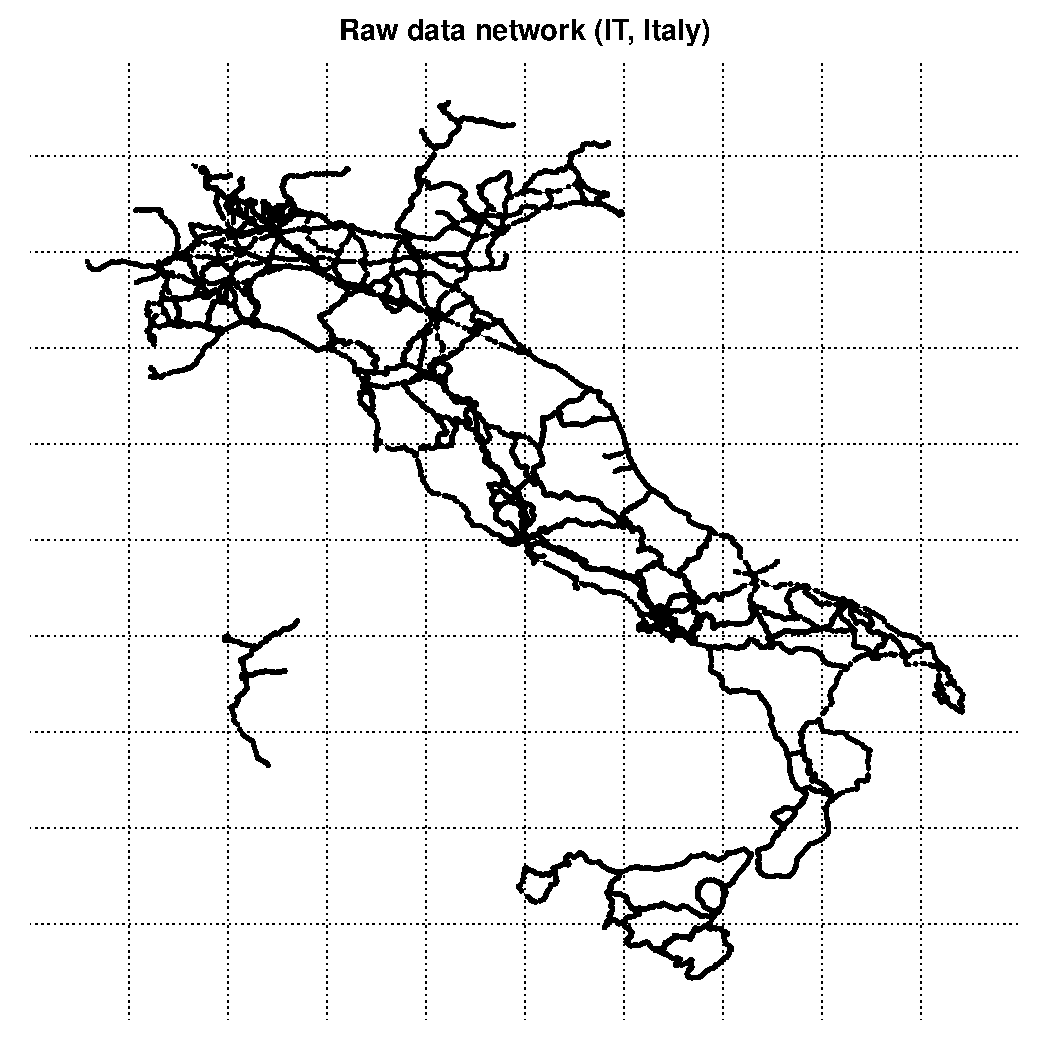
\includegraphics[width = \textwidth]{latex_source/images/railways/raw_networks/raw_IT_network.pdf}
    \label{fig:raw}
\end{minipage}



\section{Creation of the city/railways networks}
The creation of the raw network was straightforward; however, the refined network required a few specific steps:
\begin{enumerate}
\item Data was read from "RailrdC.shp" to create a list of city nodes\textbf{"{ICC}\_city\_nodes.csv"}. This file contains the columns: nodeID, nodeLabel, latitude, longitude, country\_name, and country\_ISO3.
\item The raw graph data "{ICC}\_raw\_nodes.csv" and "{ICC}\_raw\_edges.csv" is recovered. Attributes 'label' and 'is near city' are added to raw nodes. A raw node that matches a city's coordinates in "{ICC}\_city\_nodes.csv" within a specified threshold distance was assigned either "label" = "city\_name" and "is\_near\_city" = "empty" (if it was the best match) or "label" = "empty" and "is\_near\_city" = "city\_name".
\item The city/rails graph was derived as a subset of the current graph: for each pair of labeled nodes ('label' $\neq$ 'empty') that are within a maximum radius, the shortest paths were calculated. If a shortest path existed where all intermediate nodes were neither cities nor dangerously close to other cities, an edge was added to the final output graph.
\end{enumerate}
Then, the graph is created and saved with usual routines. Final output files are \textbf{"{ICC}\_nodes.csv"} and \textbf{"{ICC}\_nodes.csv"}.
\medskip \newline
The introduction of the "is\_near\_city" field was necessary because rail bifurcations often start slightly before or after entering a city station. In reality, the train must pass through the city station even if it takes the bifurcation. Without the "is\_near\_city" field, non-existent edges would be erroneously created (see figure \ref{fig:pescara_area}). The maximum radius parameter for checking edges only between sufficiently close cities was crucial for speeding up computations, especially in countries with a high number of stations and densely connected railways, such as Poland. Both threshold parameter for city matching in \textbf{flexible\_matching} and maximum radius have to be tuned after looking at the raw data.
\begin{figure}[H]
    \centering
    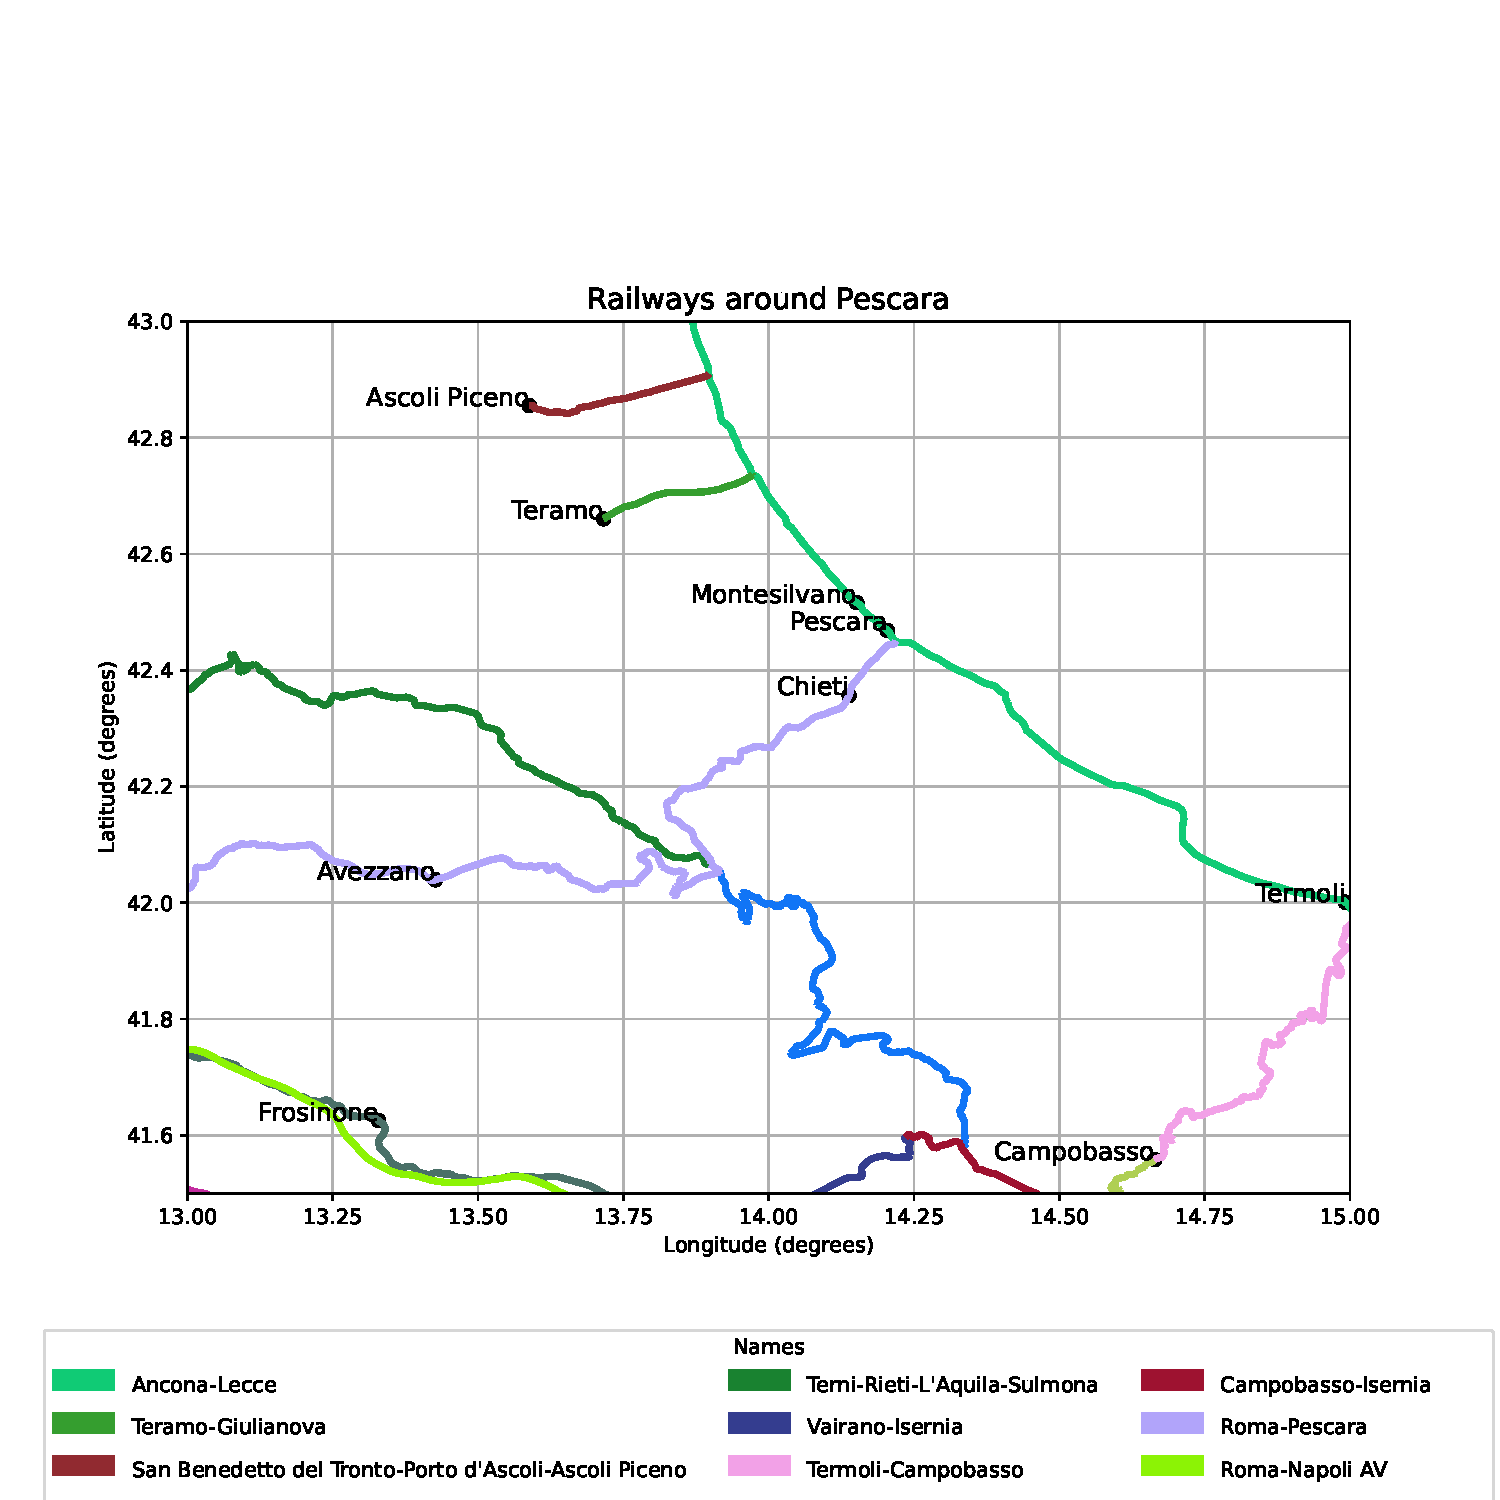
\includegraphics[width= \textwidth]{latex_source/images/railways/pescara_area.pdf}
    \caption{An example to justify the need for the "is near city" check: a rail bifurcation starts just before entering Pescara from south. Without the check implementation, edge "Termoli-Chieti" is created whereas in reality it does not exist: one wanting to get to Chieti must first get to Pescara, then take another train to Chieti. }
    \label{fig:pescara_area}
\end{figure}
\newpage
\section{Results Visualization}
\begin{figure}[H]
\centering
    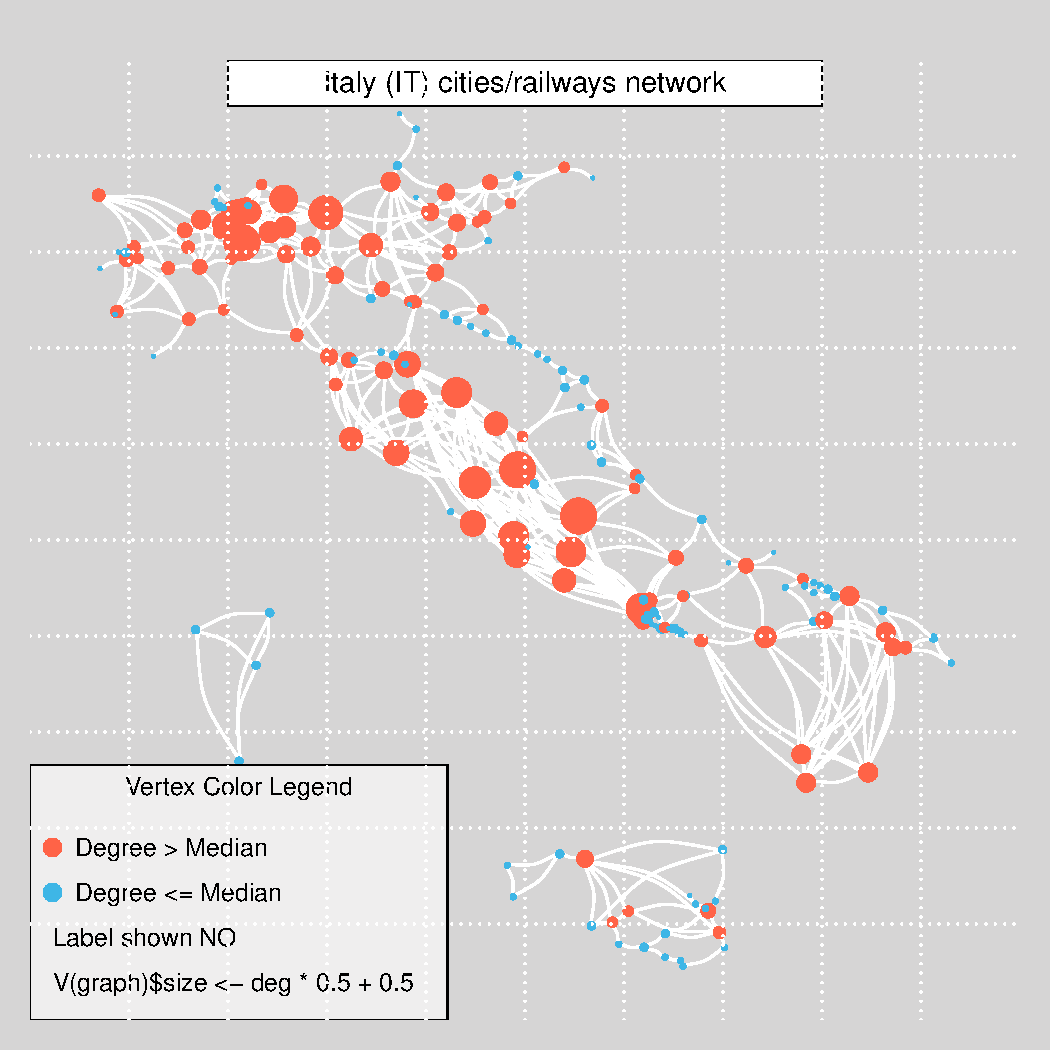
\includegraphics[width = 0.7\textwidth]{latex_source/images/railways/city_networks/IT_network.pdf}
\begin{comment}
IT (Italy) cities/ railways networks. Note the high density of edges in the center-left zone of the graph: it is a consequence of the fact that the stations "Roma Termini" and "Roma Tiburtina" are missing from file "RailrdC.shp". Many stations result directedly connected where in reality they are not because Rome stations are in between.
\end{comment}

\begin{subfigure}{}
    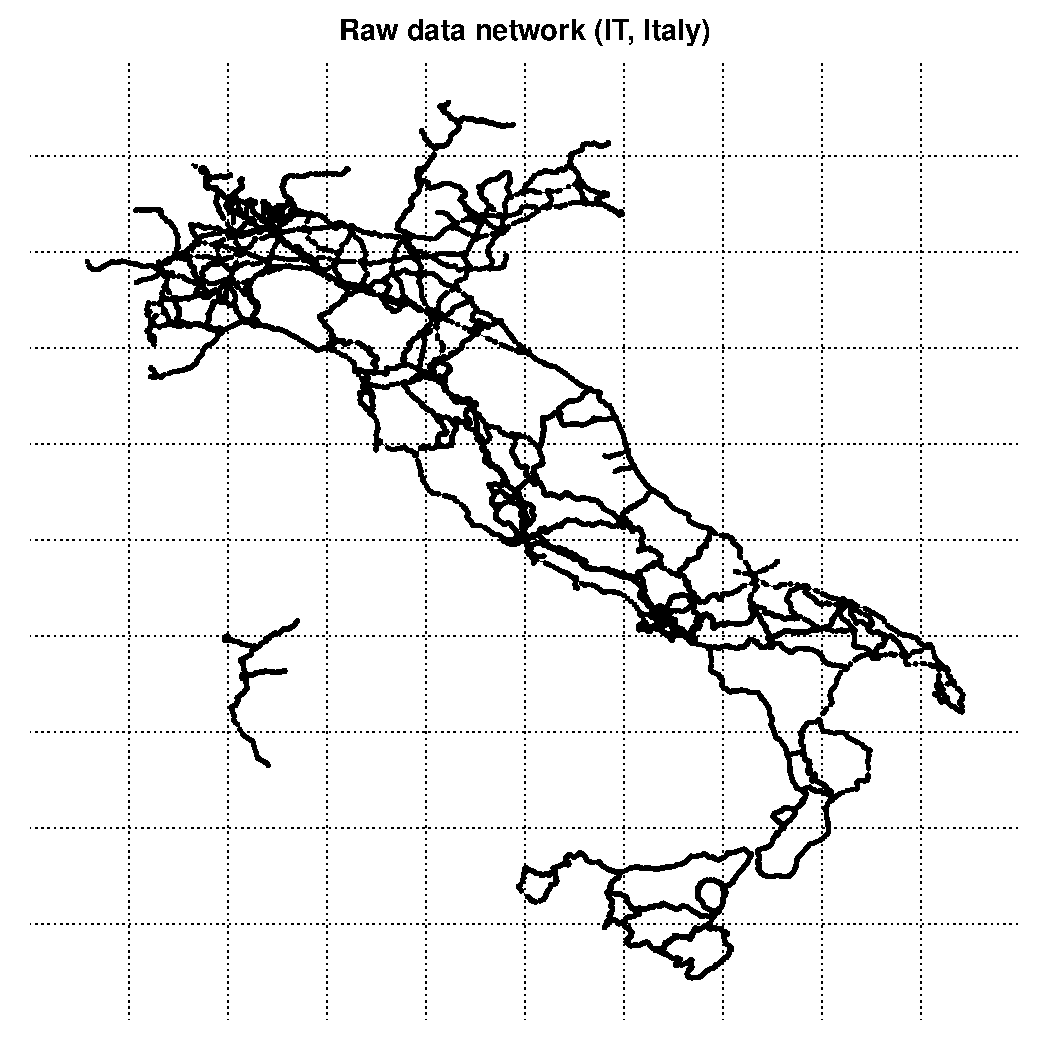
\includegraphics[width = 0.3\textwidth]{latex_source/images/railways/raw_networks/raw_IT_network.pdf}
\end{subfigure}
\begin{subfigure}{}
    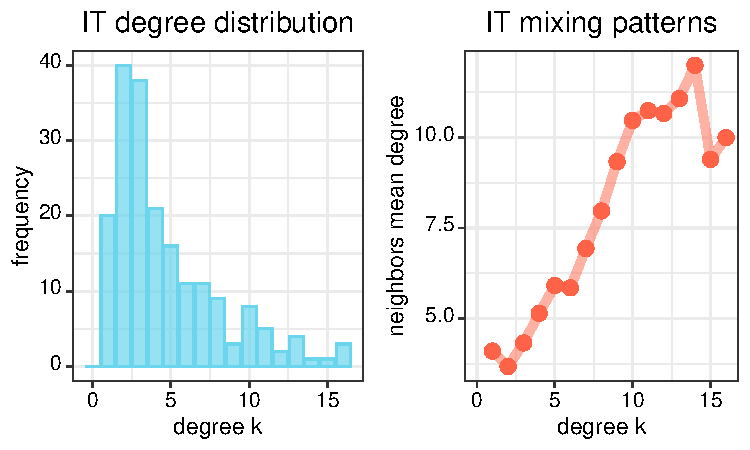
\includegraphics[width = 0.6\textwidth]{latex_source/images/railways/city_network_analysis/IT_analysis.pdf}
\end{subfigure}
\caption{}
\end{figure}
\newpage
\subsection*{Appendix}
\addcontentsline{toc}{section}{Appendix}
\subsection*{Supplementary Figures}
\begin{figure}[H]
    \centering
    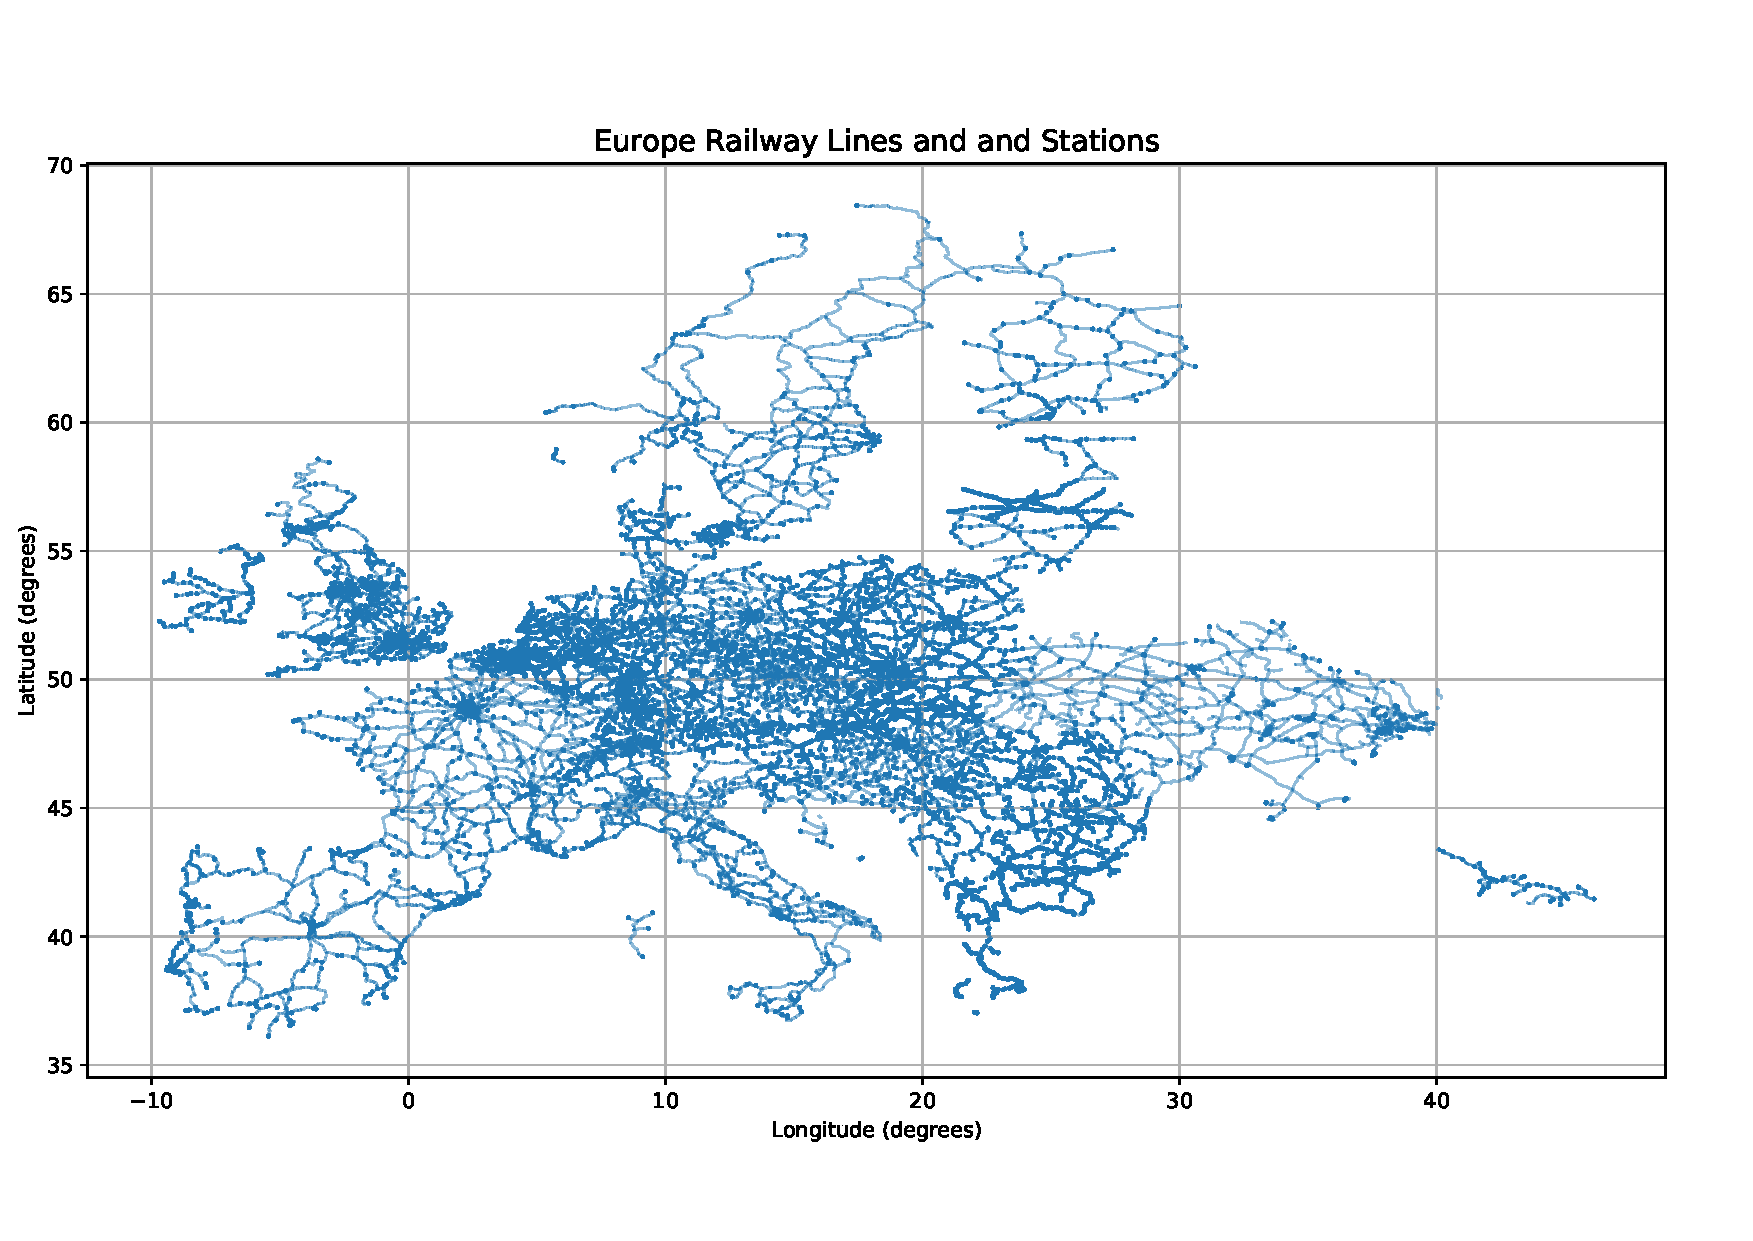
\includegraphics[width = 0.8 \textwidth]{latex_source/images/railways/europe.pdf}
    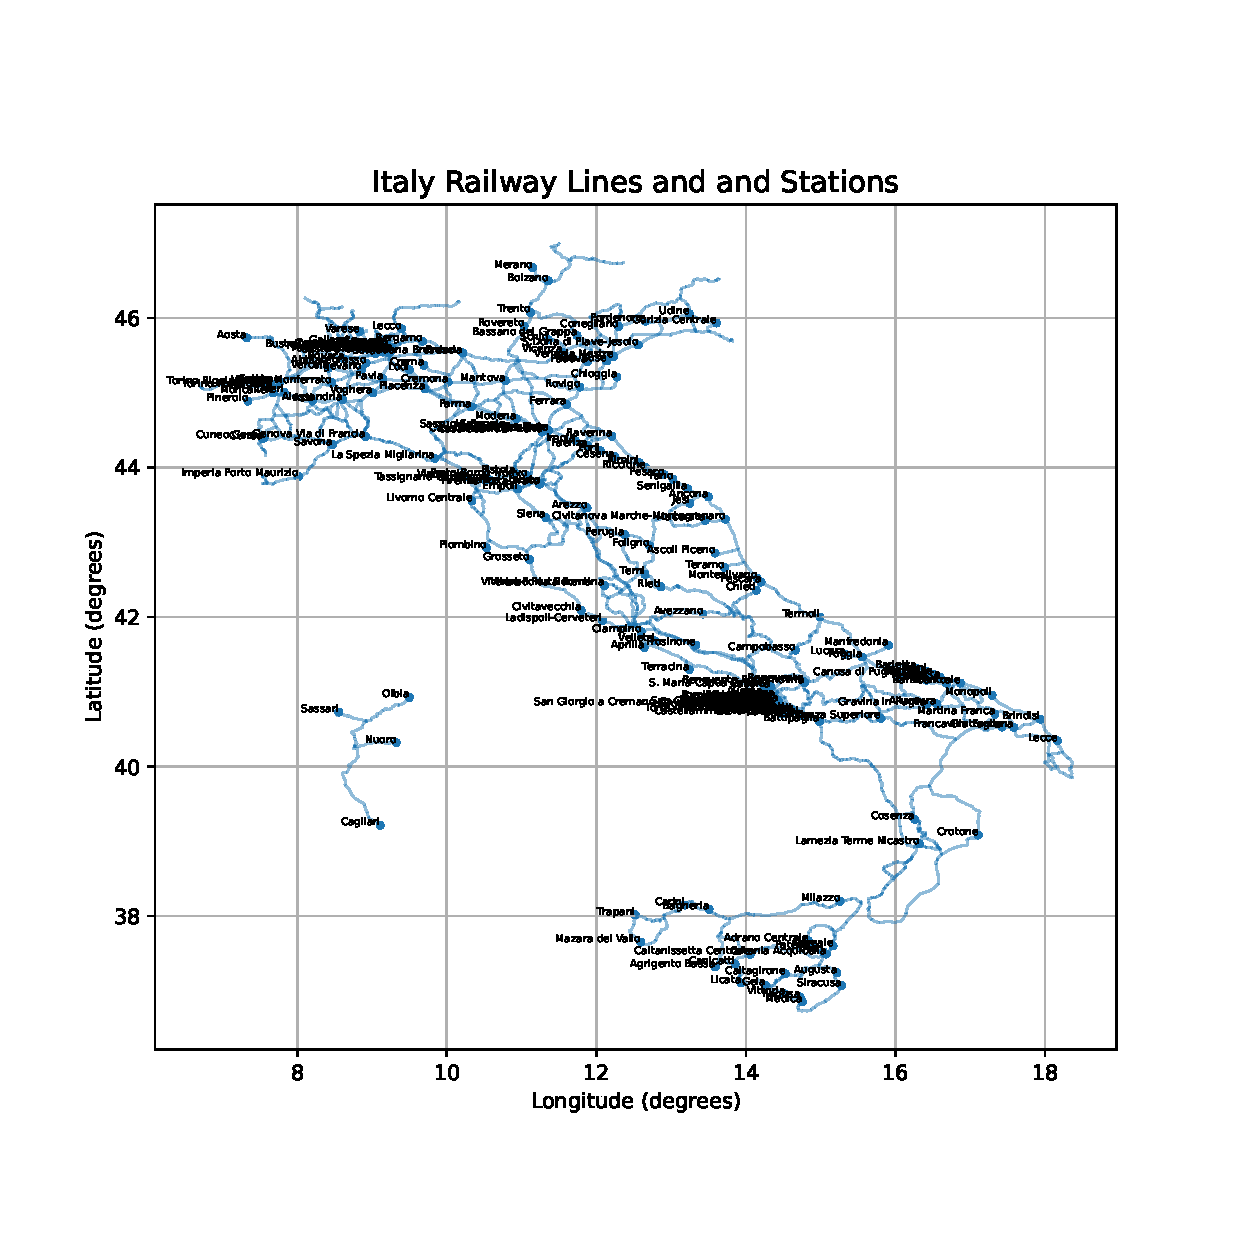
\includegraphics[width = 0.7\textwidth]{latex_source/images/railways/italy.pdf}
    \caption{\textbf{Top}: Railways and stations of the whole Europe. Each dot (line, respectively) is an element of the dataframe stations (railways, respectively). Only operational lines (EXS code $= 28$) have been filtered out. \textbf{Bottom}: A zoom on Italy. We can already see by eye that data is incomplete (for instance,stations of Verona, Trieste and Roma are missing form the chart). Also, in the metropolitan area of Napoli there is a high density of stations, because also the smallest ones are reported in the database, whereas for other areas of Italy (like Veneto) only the biggest stations are reported. We cannot thus expect to recover a very accurate network of railways from this dataset.}
\label{fig:rails_preliminary}
\end{figure}
